\section{Related Work} \label{related work}

% why do we need tuning?
% To achieve peak performance and power efficiency for scientific applications on today's HPC machines, it is necessary to tune various compile-time and runtime configurations.
%On one side, configurations such as compile-time optimizations, runtime library parameters, and architectural configurations, may have a significant impact \cite{iterativecompilation, Chen:2010:EIO:1806596.1806647, powerTuner, energyTuner, cluster2016, sc2017}.
%On the other side, settings effective for one program/machine combination may not achieve peak performance on another, and it is both tedious and challenging to manually find the best configuration \cite{sc04oliver}.
%To attain the best performance, it is vital to automate the space exploration in an efficient manner.

% overview
 The first order objective of compiler-based auto-tuning techniques \cite{Hall:2009:CRN:1461928.1461946,grandstrand:2004} is performance, while the second order objectives are code size, power draw, and energy consumption.
 We divide prior work into the following two categories

\vspace{.25em}
\noindent (1) Compiler flag selection techniques \cite{1611551,PanE06,iterativecompilation,Cavazos:2007:RSG:1251974.1252540, Pan:2008:taco, cere, cern2012,Chen:2010:EIO:1806596.1806647, Vaswani:2007:MSE:1251974.1252536, Kulkarni:2004:FSE:996841.996863, 4625477}:
given a set of compiler flags, the objective is to determine the combination that generates the most performant executable on a given architecture.
Our work and many related papers \cite{Chen:2010:EIO:1806596.1806647, cere,PanE06,Pan:2008:taco} belong to this category.
\cite{Pan:2008:taco, cere} also take a fine-grained per-region approach.
They select the best code variant for each region in a greedy fashion without
considering interactions among different code variants; this is is effective for
their case studies but results in  worse performance than random search
for OpenMP-based scientific applications.
To reduce the overhead of search-based approaches, researchers have also proposed
schemes based on machine learning techniques \cite {1611549, Cavazos:2007:RSG:1251974.1252540, cobayn}.
As the state-of-the-art, COBAYN \cite{cobayn} infers good compile flags for a new program by representing them as static/dynamic features to a pre-trained Bayesian network.
Our experimentation shows that FuncyTuner outperforms COBAYN for Intel compiler
while incurring similar cost.

\begin{figure}
\centering
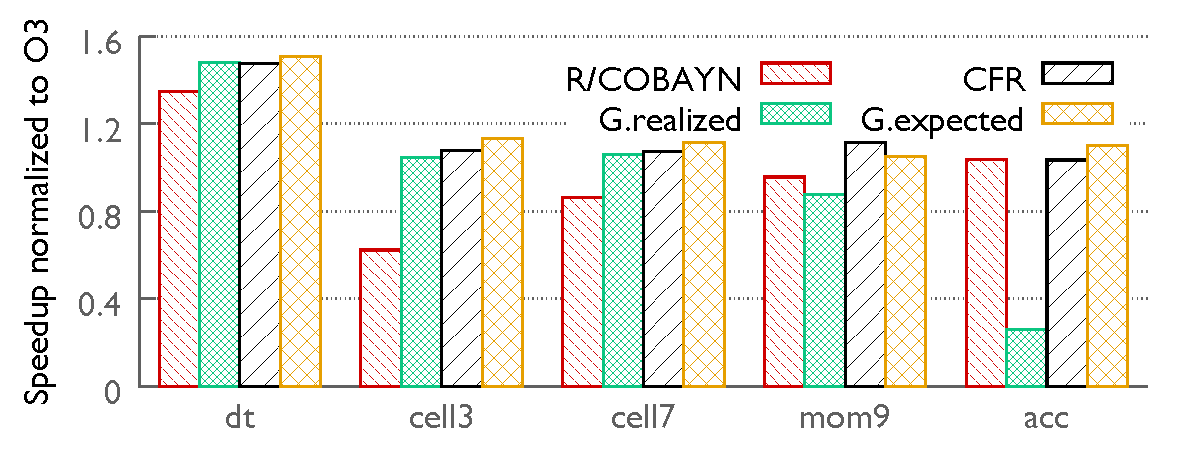
\includegraphics[width=0.6\textwidth]{gnuplot_temp/deep_dive.pdf}
\vspace{-6mm}
\caption{Normalized speedups for top-5 loops of Cloverleaf on Intel Broadwell.
Note: COBAYN (static) and R generated the same code in this case.}
\label{fig:case}
\vspace{-4mm}
\end{figure}


\vspace{.25em}
\noindent (2) Compiler phase ordering techniques \cite{Kulkarni:2012:MCO:2384616.2384628, Nobre:2016:GIC:2907950.2907959, Kulkarni:2004:FSE:996841.996863, 6662511, micomp}:
given a set of compiler optimization passes, there are many valid orders to apply each of them, which usually generate code variants with different runtime performance.
Our work focuses on the Intel tool chain, which does not provide command-line flags to perform phase ordering.
However, our approach may be applicable to Clang/LLVM, which supports such capability.
We plan to explore this in future work.


\begin{comment}
% search-based, random and genetic search
Random methods \cite{Chen:2010:EIO:1806596.1806647,opentuner} evaluate and select the best combination out of many randomly drawn in a uniform manner from the search space.
Chen et al. \cite{Chen:2010:EIO:1806596.1806647} conduct an in-depth study on a fundamental question of iterative compilation with random space search, i.e., program input sensitivity, with 1000 data sets for each benchmark.
They observe that a single optimization flag combination can achieve most of the best performance for a program across all the data sets for their benchmark suites.
So far, we do not consider input sensitivity as our primary objective, but we plan to look into it in the future.
Genetic algorithms \cite{Kulkarni:2004:FSE:996841.996863, 4625477} can also be used to search the flag combination space.
However, due to relatively high search overhead and resource limitations, we do not explore them in this work. Also, we consider our current approach to be more intuitive so that our results are easier to interpret that those derived from genetic algorithms that act as a black box.

% search-based, previous state-of-the-art
Pan et al. \cite{1611551} propose Combined Elimination (CE) to capture interactions among GCC compiler optimizations.
CE starts off with all compiler optimizations and eliminates those that introduce negative performance impacts in a greedy and iterative fashion.
It considers all 38 on/off flags of GCC 3.3.3 and treats a program as a whole.
Their experiments show CE effectively reduces the tuning overhead while achieving comparable performance results to prior approaches \cite{1191546, 1348305}.
In contrast, we take a fine-grained per-loop approach for both binary and multi-valued flags for latest Intel C/C++ Compiler tool chain.
Our evaluation also indicates CE performs worse than our approach.
\end{comment}

%and is not comparable to ours, either.
%Taken CE as the state-of-the art,
\begin{comment}
Cavazos et al. \cite{Cavazos:2007:RSG:1251974.1252540} show that CE is neither effective nor efficient for the EKOPath commercial compiler with 121 optimizations and is also worse than a random selection method, which is consistent with our experimental evaluations for ICC.
\end{comment}
% automated predictive modeling

\begin{comment}
Given a new program, CE tries to exploit the interactions among compiler optimizations implicitly with no reuse of prior knowledge, while machine learning techniques \cite{1611549, Cavazos:2007:RSG:1251974.1252540} build a model representing the prior knowledge to reuse for new applications.
Agakov et al. \cite{1611549} proposed two probabilistic models for a set of training programs.
The model can use an independent and identical distribution (IID) or a stationary Markov chain, which is learned by simply counting the occurrences of desired sub-sequences in the training optimization sequences.
Given a new program, their approach first extracts its static features and applies nearest-neighbor search to determine which learned probabilistic model is the best fit.
During the tuning stage, the desired number of samples can be drawn from the model.
Their experiments show that their approach can find good optimization sequences faster than a pure random search and genetic algorithm based search.
Cavazos et al. \cite{Cavazos:2007:RSG:1251974.1252540} collect hardware performance counters as feature sets to train a probabilistic model for optimization sequence selection.
Their work demonstrates the importance of using dynamic program features and a learned statistical model for prior knowledge in compiler optimization selection.
They also note that static features used in their previous work \cite{1611549} for small embedded kernel benchmarks are not effective for large applications with many dynamic branches.
We want to highlight that although predictive models \cite{1611549, Cavazos:2007:RSG:1251974.1252540} reduce tuning overhead, they do not improve the best achievable performance by random search while our approach does perform better and has the potential to improve these predictive models.
\end{comment}

\iffalse
% more automated predictive modeling
Modeling techniques have also employed logistic regression, neural network and multivariate adaptive regression splines \cite{Vaswani:2007:MSE:1251974.1252536, Cavazos:2007:RSG:1251974.1252540}, Bayesian networks \cite{6962349}, dependency trees \cite{Garciarena:2016:EOC:2908961.2931696}, probabilistic graphs \cite{Nobre:2016:GIC:2907950.2907959}, and stationary Markov chains \cite{1611549}.
These methods all try to implicitly capture the interactions and dependencies among compiler flags or compilation phases in order to focus search on the area with highest performance potential.
Program features can be estimated statically \cite{1611549} or dynamically with performance counters \cite{Cavazos:2007:RSG:1251974.1252540, 6962349, Leather:2009:AFG:1545006.1545059}.
%, and may be automatically extracted \cite{}.
Instead of utilizing program features to build models, our approach simply relies on per-loop time collected by light-weighted Caliper \cite{caliper} to implicitly capture the interactions of compiler flags on different compilation modules.
This relieves programmers from having to build complicated models before obtaining performance benefits for their target programs.
Moreover, a recent study \cite{FursinMGL15} utilizing crowd-sourcing compilation shows accuracy for machine-learning predictive models on large-scale datasets is close to that of a random guess.
Such a surprising result also raises a fundamental concern about machine-learning based approaches, namely, scarcity of training data, meaningful features, and validity of generalization, in addition to an inherent difficulty in interpreting learned models.
\fi

\iffalse
% manual predictive modeling
The interaction of compiler flags or phases can also be captured explicitly with expert knowledge.
Jantz et al. \cite{6662511} manually classified VPO optimization phases into cleanup phases, branch phases and non-branch phases.
After verifying the independence among branch phases and non-branch phases, they divide the phases into two disjoint groups and show extreme effectiveness of utilizing phase interaction information to reduce the search space size by 96.75\% while achieving almost the same performance as previous search-based techniques.
However, such an expert characterization process is very time consuming and may not be feasible for production quality compilers like ICC, GCC and LLVM, while our method is readily applicable.
\fi

\begin{comment}
% Domain-specific and architecture-specific tuning
The aforementioned compiler-based tuning techniques are general in the sense they do not take advantage of domain knowledge of programs being tuned.
Zhang et al. \cite{frank2012, frank2013} propose an auto-tuner for 3D stencil code generation on several heterogeneous GPUs.
They exhaustively search a space composed of GPU thread block dimensions and memory placement.
In \cite{5161004, Tiwari:2009:SAF:1586640.1587552}, Tiwari et al. propose a domain-specific language (DSL) for compilation transformation recipes.
Their framework tunes each computation kernel separately and requires experts to write valid recipes in their DSL while our framework tunes multiple kernels simultaneously via compiler command-line flags, a process that can be fully automated.
\end{comment}

\iffalse
% others
Sourouri et al. \cite{sc2017} employ dynamic voltage and frequency scaling (DVFS) on Intel Xeon multi-core machines to tune each kernel of their seismic wave propagation application.
They exhaustively search a space composed of core and uncore frequency, number of OpenMP threads and then enforce the best per-kernel configuration via runtime library for energy-saving.
Others have also investigated runtime adaption techniques to account for performance discrepancies incurred by power caps \cite{cluster2016} or to impose different tuning objectives.
%that can be indiuser's disposal.
Our approach focuses on compile-time flag composition and is orthogonal to their work.
\fi
